\documentclass[journal,twoside,web]{ieeecolor}
\usepackage{generic}
\usepackage{cite}
\usepackage{amsmath,amssymb,amsfonts}
\usepackage{algorithmic}
\usepackage{graphicx}
\usepackage{algorithm,algorithmic}
\usepackage{hyperref}
\hypersetup{hidelinks=true}
\usepackage{textcomp}
\usepackage{caption}
\usepackage{subfigure}
\usepackage{listings}

% Farben für die Syntax-Hervorhebung definieren
\definecolor{codegreen}{rgb}{0,0.6,0}
\definecolor{codegray}{rgb}{0.5,0.5,0.5}
\definecolor{codepurple}{rgb}{0.58,0,0.82}
\definecolor{backcolour}{rgb}{0.95,0.95,0.92}

% Stil für Java festlegen
\lstdefinestyle{javastyle}{
    language=Java,
    basicstyle=\ttfamily\scriptsize, 
    breaklines=true,                 
    breakatwhitespace=true,          
    postbreak=\mbox{\textcolor{red}{$\hookrightarrow$}\space},
    tabsize=2,                       
    numbers=left,
    numbersep=5pt,
    xleftmargin=15pt,                
    framexleftmargin=15pt,           
    frame=none
}


\lstset{style=javastyle}

\captionsetup[figure]{justification=centering}
\def\BibTeX{{\rm B\kern-.05em{\sc i\kern-.025em b}\kern-.08em
    T\kern-.1667em\lower.7ex\hbox{E}\kern-.125emX}}
\markboth{\hskip25pc Lindenmayer-Systeme }
{Lindenmayer-Systeme}
\begin{document}
\title{Lindenmayer-Systeme-Test}
\author{\parbox{\textwidth}{\centering Dana Lenzig, Luise Schäffel, Lea Vianne Eichler}}

\maketitle

\begin{abstract}
These instructions give you guidelines for preparing papers for 
IEEE Transactions and Journals. Use this document as a template if you are 
using \LaTeX. Otherwise, use this document as an 
instruction set. The electronic file of your paper will be formatted further 
at IEEE. Paper titles should be written in uppercase and lowercase letters, 
not all uppercase. Avoid writing long formulas with subscripts in the title; 
short formulas that identify the elements are fine (e.g., "Nd--Fe--B"). Do 
not write ``(Invited)'' in the title. Full names of authors are preferred in 
the author field, but are not required. Put a space between authors' 
initials. The abstract must be a concise yet comprehensive reflection of 
what is in your article. In particular, the abstract must be self-contained, 
without abbreviations, footnotes, or references. It should be a microcosm of 
the full article. The abstract must be between 150--250 words. Be sure that 
you adhere to these limits; otherwise, you will need to edit your abstract 
accordingly. The abstract must be written as one paragraph, and should not 
contain displayed mathematical equations or tabular material. The abstract 
should include three or four different keywords or phrases, as this will 
help readers to find it. It is important to avoid over-repetition of such 
phrases as this can result in a page being rejected by search engines. 
Ensure that your abstract reads well and is grammatically correct. 
\end{abstract}

\section{Einleitung}

\subsection{Problemstellung und Motivation}

\subsection{Ziel}

\section{Theoretische Grundlagen}

\subsection{Funktionsweise von Lindenmayer-Systemen}

\subsection{Produktionsregeln und Iterationen}

\subsection{Grafische Interpretation mittels Turtle-Grafik}

\section{Konzeption und Implementierung}

\subsection{Aufbau der Simulation}

\subsection{Implementierung der Produktionsregeln}

\subsection{Visualisierung der generierten Strukturen}

\section{Ergebnisse und Diskussion}

\subsection{Darstellung ausgewählter Simulationsergebnisse}

\subsection{Einfluss von Parametern auf die Ergebnisse}

\subsection{Grenzen der Simulation}

\section{KI-Einsatz und Fazit}

\subsection{Einsatz von KI während der Entwicklung}

\subsection{Zusammenfassung und Ausblick}

\subsection{Referenz auf externen BibTex-Eintrag}

Hier sieht man ein Zitat: \cite{schluessel_jahr}

\subsection{Bilder}

\begin{figure}[h]
    \centering
    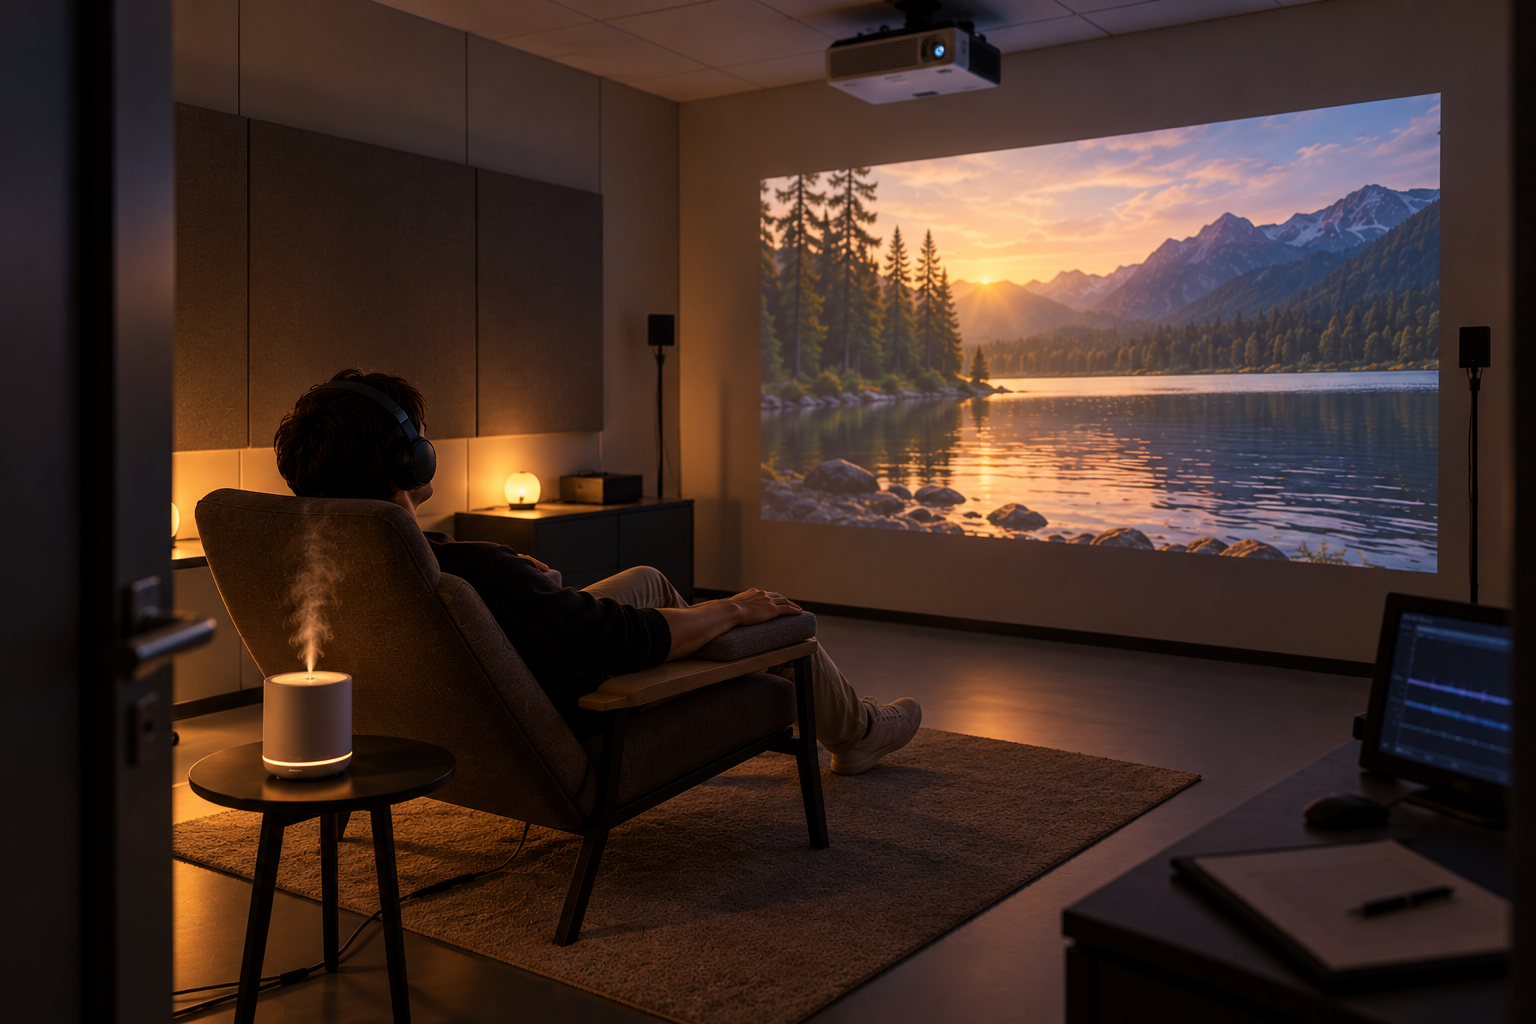
\includegraphics[width=0.5\textwidth]{img/image.png}
    \caption{Bildbeschreibung}
\end{figure}


\begin{figure}[h]
    \centering
    \subfigure[Beschreibung Bild1]{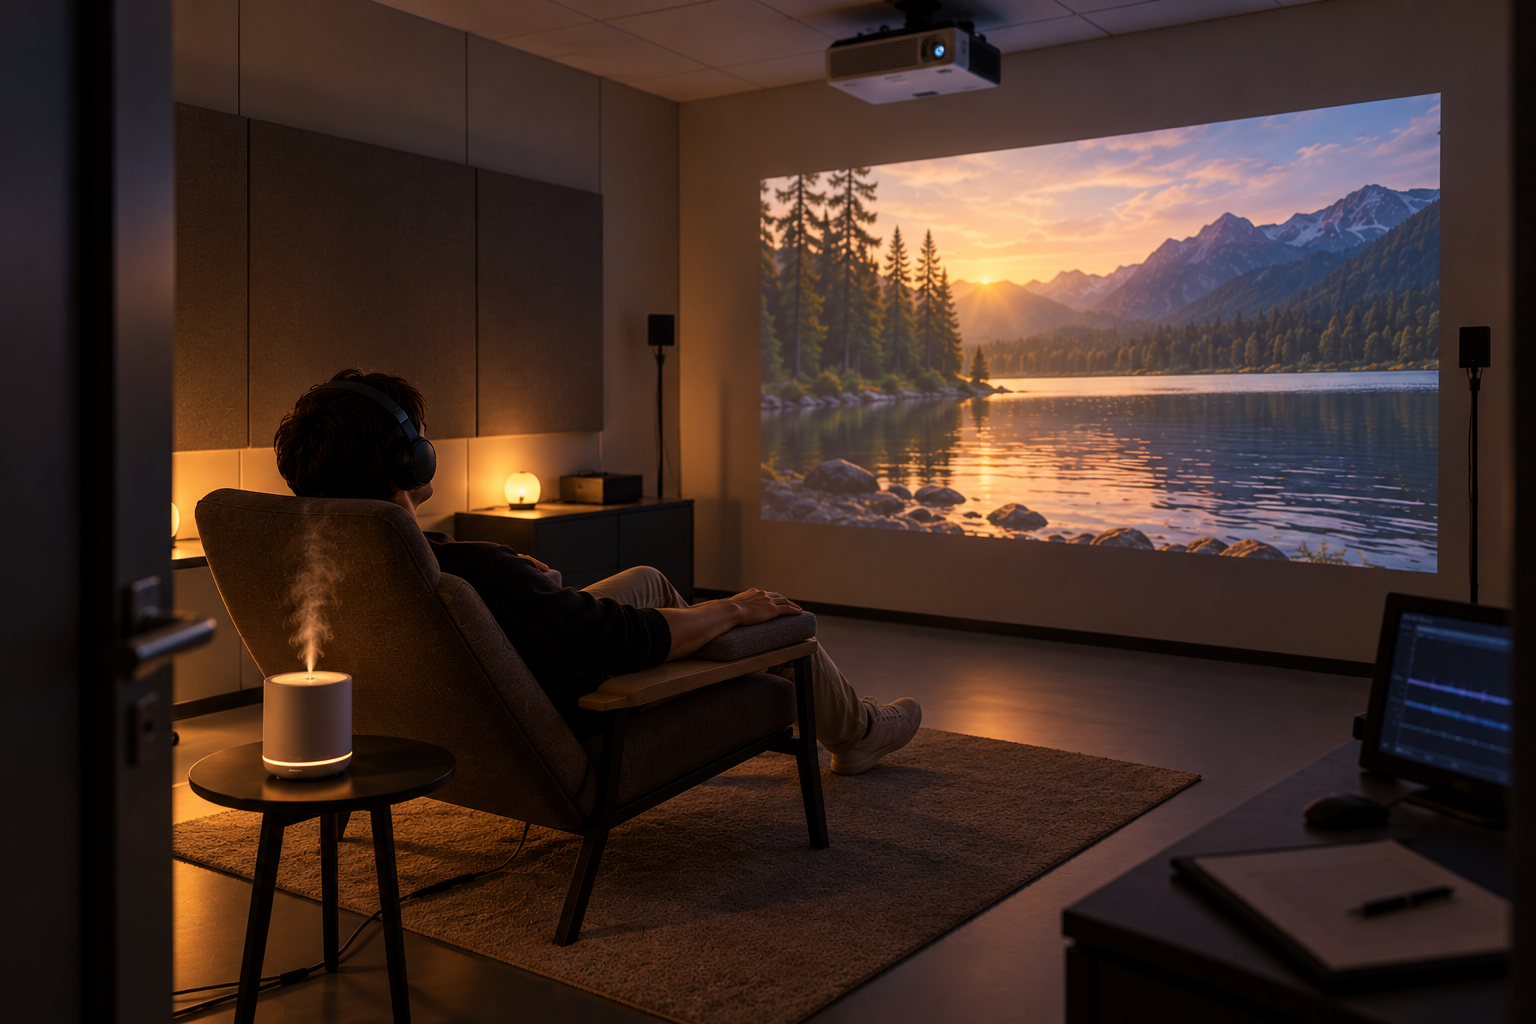
\includegraphics[width=0.24\textwidth]{img/image.png}}
    \subfigure[Beschreibung Bild2]{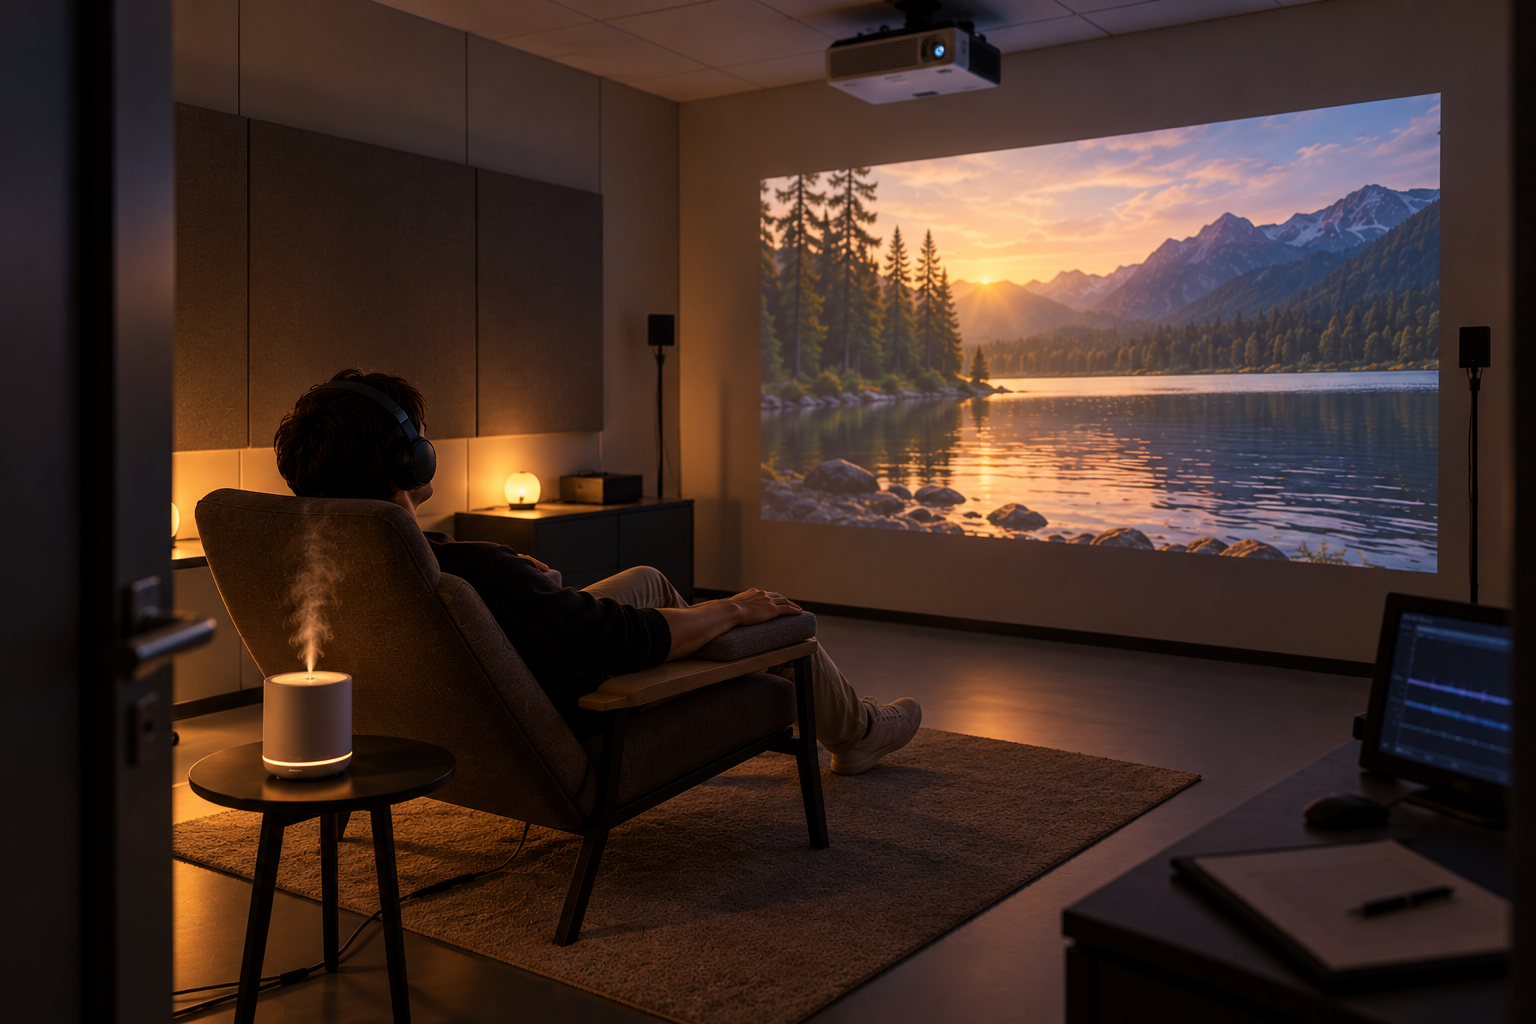
\includegraphics[width=0.24\textwidth]{img/image.png}}

    \caption{Zwei Bilder nebeneinander}
    \label{fig:labeltest}
\end{figure}

\subsection{Referenz auf Bild}

Referenziere ein Bild über \ref{fig:labeltest}

\subsection{Quellcode (hier auf Java vorkonfiguriert)}

\begin{lstlisting}[language=Java]
public class HelloWorld {
    public static void main(String[] args) {
        // Gibt eine Nachricht auf der Konsole aus
        System.out.println("Hallo Welt!");
    }
}
\end{lstlisting}

\newpage

\section{References}
\bibliographystyle{IEEEtran}
\bibliography{references}
\end{document}
